\documentclass[]{standalone} 
\usepackage{pgfplots} 
%\usepgfplotslibrary{external} 
%\tikzexternalize 
\usepgfplotslibrary{fillbetween}
\usepackage{tikz} 
\usepackage{amsmath} 
\usepackage{pgfplots} 
\usetikzlibrary{calc} 
\pgfplotsset{compat = newest, every axis plot post/.style={line join=round}, label style={font=\Large} }
\begin{document} 
	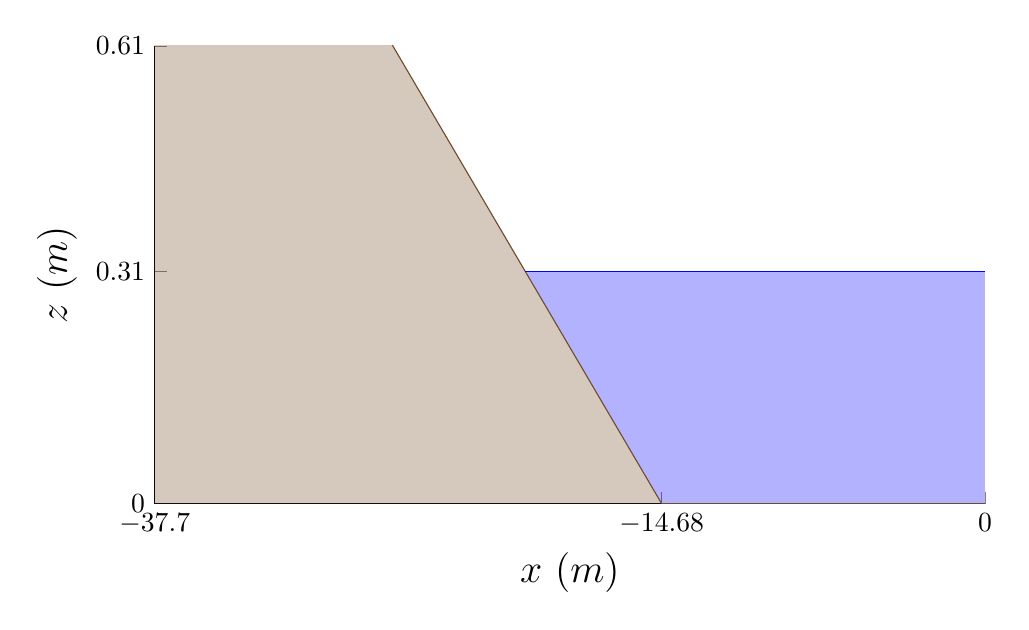
\begin{tikzpicture}
	\begin{axis}[ 
	width = \textwidth,
	height = 0.61\textwidth,
	axis y line*=left,
	axis x line*=bottom, 
	xtick={0,-14.68,-37.7},  
	ytick = {0,0.3097,0.61}, 
	xmin=-37.7, 
	xmax=0, 
	ymin =0, 
	ymax = 0.61,
	xlabel=$x$ ($m$), 
	ylabel=$z$ ($m$)]
	
	\addplot [name path=b,brown!60!black] coordinates {(0,0) (-14.68,0)  (-37.7,1.15)};
	
	\path[name path=axis] (axis cs:0,0) -- (axis cs:-37.7,0);
	
	\addplot [name path=a,blue] coordinates {(0,0.3097) (-20.9,0.3097)};
	
		\addplot [
		thick,
		color=brown!60!black,
		fill=brown!60!black, 
		fill opacity=0.3
		] fill between[of=b and axis];
		
	\addplot [
	thick,
	color=blue,
	fill=blue, 
	fill opacity=0.3
	] fill between[of=a and b];
	

	\end{axis} 
	
	
	
	\end{tikzpicture}
\end{document}